% vim: set tw=78 tabstop=4 shiftwidth=4 aw ai:
\documentclass{beamer}

\usepackage[utf8x]{inputenc}		% diacritice
\usepackage[english]{babel}
\usepackage{color}			% highlight
\usepackage{alltt}			% highlight
\usepackage{caption}
\usepackage{frame}


% highlight; comment this out in case you don't input code source files
%\usepackage{code/highlight}		% highlight
\usepackage{hyperref}			% folosiți \url{http://...}
					% sau \href{http://...}{Nume Link}
\usepackage{verbatim}

\mode<presentation>
{ \usetheme{Berlin} }

% Încărcăm simbolurilor Unicode românești în titlu și primele pagini
\PreloadUnicodePage{200}

% Arătăm numărul frame-ului
\newcommand{\frameofframes}{/}
\newcommand{\setframeofframes}[1]{\renewcommand{\frameofframes}{#1}}

\setframeofframes{of}
\makeatletter
\setbeamertemplate{footline}
  {%
    \begin{beamercolorbox}[colsep=1.5pt]{upper separation line foot}
    \end{beamercolorbox}
    
    \begin{beamercolorbox}[ht=2.5ex,dp=1.125ex,%
      leftskip=.3cm,rightskip=.3cm plus1fil]{title in head/foot}%
      {\usebeamerfont{title in head/foot}\insertshorttitle}%
      \hfill%
      {\usebeamerfont{frame number}\usebeamercolor[fg]{frame number}\insertframenumber~\frameofframes~\inserttotalframenumber}
    \end{beamercolorbox}%
    \begin{beamercolorbox}[colsep=1.5pt]{lower separation line foot}
    \end{beamercolorbox}
  }
\makeatother

\setbeamertemplate{navigation symbols}{}%remove navigation symbols

\title[Deep models used in games]{Deep models used in games}
\subtitle{Bachelor Thesis Session -- September 2015}
\institute{Faculty of Automatic Control and Computers,\\
	University POLITEHNICA of Bucharest}
\author[Florentina-Ștefania Bratiloveanu]{Florentina-Ștefania Bratiloveanu\\
	Supervisor: As. Drd. Ing Tudor Berariu}
\date{September 14, 2015}

\begin{document}

% Slide-urile cu mai multe părți sunt marcate cu textul (cont.)
\setbeamertemplate{frametitle continuation}[from second]

\frame{\titlepage}

\frame{\tableofcontents}

% NB: Secțiunile nu sunt marcate vizual, ci doar apar în cuprins


%--------------------MOTIVATION--------------------	
\section{Motivation}
\begin{frame}{Motivation}
	\begin{itemize}
		\item de
		\item find models capable of generalization
	\end{itemize}
\end{frame}

\section{State of the art}
%--------------------INTRODUCTION--------------------	
\begin{frame}{Once upon a time...}
	\begin{itemize}
		\item reinforcement learning: Q-Learning
		\item neural networks \textbf{vs} deep neural networks
	\end{itemize}
	\centering
	\includegraphics[width=205px,height=130px]{img/nn2}
\end{frame}

%--------------------PREPROCESSING, MODEL, LOSS FUNCTION--------------------	
\begin{frame}{PREPROCESSING, MODEL, LOSS FUNCTION}
	\begin{itemize}
		\item color space: RGB, YUV, grayscale
		\item data normalization 0..1, contrast normalization
		\item activation functions
		\begin{itemize}
			\item hidden layer vs output layer
			\item tanh, sigmoid, ReLU
		\end{itemize}
		\item how many layers/features, what type of layers
		\item loss function: classification(binary/multi-class) or regression?
	\end{itemize}
\end{frame}

%--------------------TRAINING AND TESTING--------------------	
\begin{frame}{Train and test}
	\begin{itemize}
		\item split dataset for training and testing
		\item when to stop training?
	\end{itemize}
	 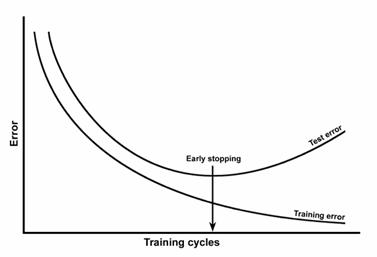
\includegraphics[width=180px,height=123px]{img/traintest.jpg}
\end{frame}

\section{Architecture, Design, Results}
\begin{frame}{Once upon a time...}
	\begin{itemize}
		\item Basic formula
			\begin{beamerboxesrounded}[lower=block body,shadow=true]{}
				\texttt{\#define MAX(a, b)   ((a) > (b) ? (a) : (b))}
			\end{beamerboxesrounded}
		\item TODO
	\end{itemize}
\end{frame}



\begin{frame}{Q-Learning}
	\begin{itemize}
	\item finds optimal policy for action-value function
	\item Q(s,a) = Q(s,a) + $\alpha\cdot$(r + $\gamma\cdot \max_a Q(s^\prime,a^\prime)-Q(s,a)$)
	\end{itemize}	
	\begin{figure}[hp]
\centering
\minipage{0.30\textwidth}
  \framebox{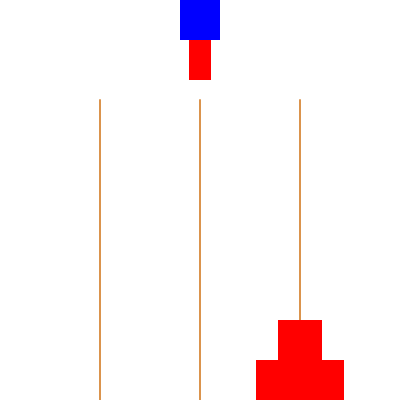
\includegraphics[width=\linewidth]{img/50}}
  \caption*{\newline UP = 90,6534\newline DOWN = 86,8787\newline LEFT = 89,1867\newline RIGHT = 94,2824}\label{fig:fa}
\endminipage\hfill
\minipage{0.30\textwidth}
  \framebox{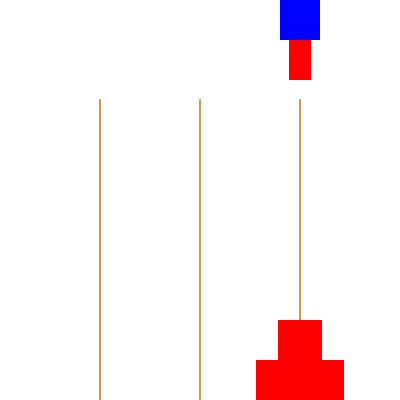
\includegraphics[width=\linewidth]{img/85}}
  \caption*{\newline UP = 97,6530\newline DOWN = 100,0000\newline LEFT = 93,8538\newline RIGHT = 92,5261}\label{fig:fb}
\endminipage\hfill
\minipage{0.30\textwidth}%
  \framebox{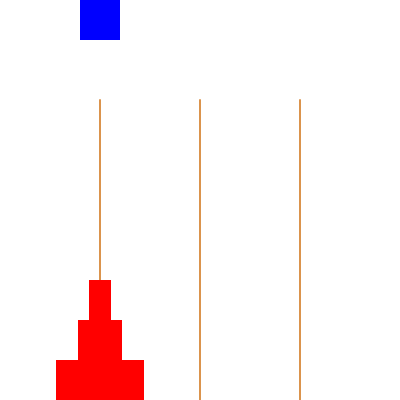
\includegraphics[width=\linewidth]{img/155}}
   \caption*{\newline UP = 26,3520\newline DOWN = 23,8452\newline LEFT = 23,8897\newline RIGHT = 22,8827}\label{fig:fc}
 
\endminipage
\end{figure}
\end{frame}


%--------------------FUTURE WORK--------------------	
\section{Future work}
\begin{frame}{Future work}
	\begin{itemize}
		\item implement Q-Network
		\item test algorithm on dynamic environments or games where the state of the universe is not fully observed
		\item make Nao capable of playing Tic-Tac-Toe
		\item after all tasks mentioned above are done, use all the information gathered for cancer classification, etc.
	\end{itemize}
\end{frame}

%--------------------CONCLUSIONS--------------------
\section{Conclusions}
\begin{frame}{Conclusions}
\begin{figure}[h]  
	\begin{minipage}[b]{0.3\textwidth}    
		
\includegraphics[width=\textwidth]{img/joke}
  	\end{minipage}
  	\hfill
  	\begin{minipage}[t]{0.55\textwidth}
		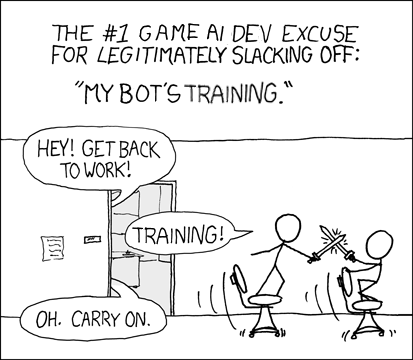
\includegraphics[width=\textwidth]{img/training}	   
	\end{minipage}
\end{figure}
\begin{flushright}
			\fontsize{5}{1em}{\texttt{Source:}} \\
			\vspace*{-0.2cm}			
			\fontsize{4}{1em}{\texttt{
			\url{http://xkcd.com/}}}
\end{flushright}	
\end{frame}

%--------------------QUESTIONS--------------------
\section{Questions}
\begin{frame}{Questions}
	\begin{center}
    \bfseries
    \Huge
    Thank you for your attention!
    
    \vspace*{1.4cm}			
    ?
  	\end{center}
\end{frame}


\end{document}
